\documentclass[12pt]{beamer} %Makes presentation

%\documentclass[handout]{beamer} %Makes Handouts
\usetheme{Singapore} %Gray with fade at top
\useoutertheme[subsection=false]{miniframes} %Supppress subsection in header
\useinnertheme{rectangles} %Itemize/Enumerate boxes
\usecolortheme{seagull} %Color theme
\usecolortheme{rose} %Inner color theme

\definecolor{light-gray}{gray}{0.75}
\definecolor{dark-gray}{gray}{0.55}
\setbeamercolor{item}{fg=light-gray}
\setbeamercolor{enumerate item}{fg=dark-gray}

\setbeamertemplate{navigation symbols}{}
%\setbeamertemplate{mini frames}[default]
\setbeamercovered{dynamics}
\setbeamerfont*{title}{size=\Large,series=\bfseries}

%\setbeameroption{notes on second screen} %Dual-Screen Notes
%\setbeameroption{show only notes} %Notes Output

\setbeamertemplate{frametitle}{\vspace{.5em}\bfseries\insertframetitle}
\newcommand{\heading}[1]{\noindent \textbf{#1}\\ \vspace{1em}}

% small footnotes
\setbeamerfont{footnote}{size=\tiny}

\usepackage{bbding,color,multirow,times,ccaption,tabularx,graphicx,verbatim,booktabs,fixltx2e}
\usepackage{colortbl} %Table overlays
\usepackage[english]{babel}
\usepackage[latin1]{inputenc}
\usepackage[T1]{fontenc}
\usepackage{lmodern}
\usepackage{alltt}

\author[]{Thomas J. Leeper}
\institute[]{
  \inst{}%
  Department of Political Science and Government\\Aarhus University
}


\title{Reproducible Research}

\date[]{October 28, 2014}

\begin{document}

\frame{\titlepage}

\frame{
    \begin{itemize}\itemsep2em
        \item<2-> \href{http://en.wikipedia.org/wiki/Growth_in_a_Time_of_Debt}{Reinhart and Rogoff}
        \item<3-> \href{http://www.slate.com/articles/health_and_science/science/2014/07/replication_controversy_in_psychology_bullying_file_drawer_effect_blog_posts.html}{Psychology's ``replication crisis''}
        \item<4-> \href{http://www.plosmedicine.org/article/info\%3Adoi\%2F10.1371\%2Fjournal.pmed.0020124}{``Most published research findings are false''}
        \item<5-> \href{http://en.wikipedia.org/wiki/Diederik_Stapel}{Diedrick Stapel}
    \end{itemize}
}


\frame{\tableofcontents}

\section{Why?}
\frame{\tableofcontents[currentsection]}

\frame{
    \frametitle{Why reproducible research?}
    \begin{itemize}\itemsep2em
        \item External reasons
        \item Internal reasons
    \end{itemize}
}

\frame{
    \frametitle{External Reasons}
    \begin{itemize}\itemsep2em
        \item<2-> Philosophical perspective
        \item<3-> Journal requirements
        \item<4-> Funding agency requirements
        \item<5-> The coming revolution
    \end{itemize}
}

\frame{
    \frametitle{Internal Reasons}
    \begin{itemize}\itemsep2em
        \item<2-> Confidence in your own work
        \item<3-> Easier workflow
        \item<4-> Easier collaboration
    \end{itemize}
}

\frame{
    \frametitle{So what does that mean?}
}


\frame{
    \frametitle{So what does that mean?}
\begin{center}
    
\includegraphics[width=\textwidth]{images/nextweek}
\end{center}
}

\frame{
    \frametitle{So what does that mean?}
    \begin{enumerate}\itemsep2em
        \item Do it for \textit{yourself} first!
        \item Do it for \textit{science} second.
    \end{enumerate}
}


\frame{
    \frametitle{Why is research still irreproducible?}
}


\frame{
    \frametitle{Why is research still irreproducible?}
\begin{center}
    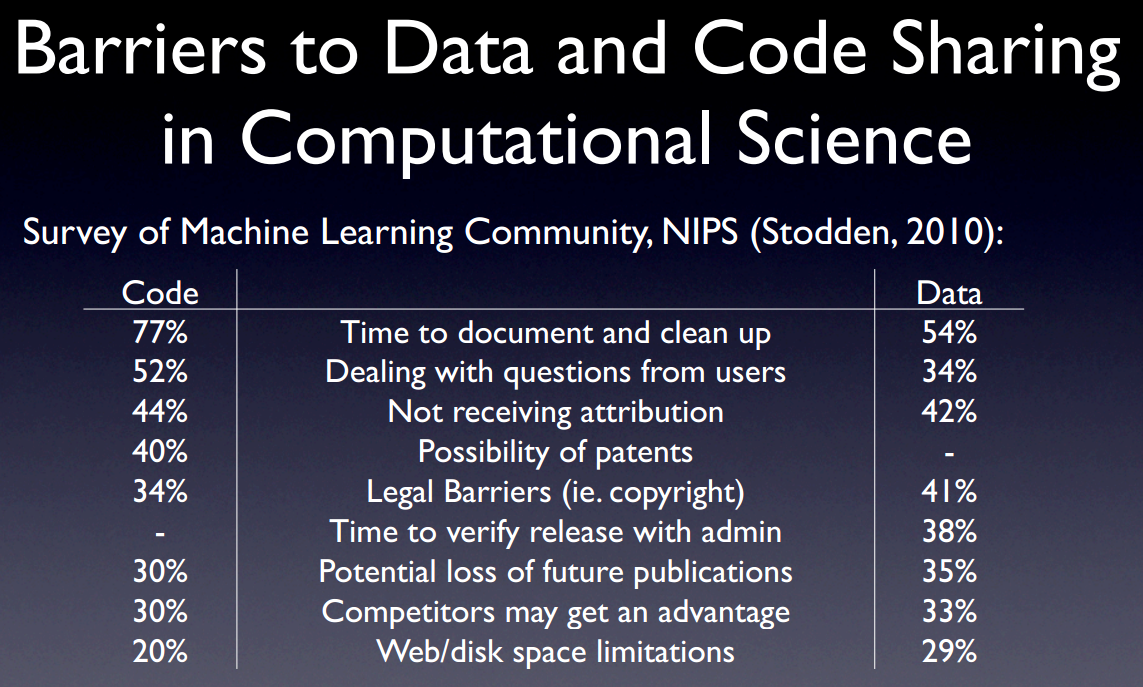
\includegraphics[width=\textwidth]{images/barriers}
\end{center}
}

\frame{
    \frametitle{Why is research still irreproducible?}
    \begin{enumerate}\itemsep2em
        \item Technology
        \item Individual actions
        \item Collective behavior and norms
    \end{enumerate}
}




\section{What?}
\frame{\tableofcontents[currentsection]}

\frame{
    \frametitle{So what is reproducible research?}
    \begin{itemize}\itemsep2em
        \item<2-> Evolving standards and technology
        \item<3-> Discipline-specific meaning
        \item<4-> Hard to define
    \end{itemize}
}


\frame{
    \frametitle{American Association for Public Opinion Research ``Disclosure Standars''}
}


\frame{
    \frametitle{American Political Science Association ``A Guide to Professional Ethics in Political Science''}
}

\frame{
    \frametitle{American Psychological Association ``Ethical Principles of Psychologists and Code of Conduct''}
}

\frame{
    \frametitle{Association for Psychological Science ``Submission Guidelines''}  
}

\frame{
    \frametitle{American Anthropological Association ``Code of Ethics''}
}

\frame{
    \frametitle{CONSORT Group ``CONSORT Statement''}
}


\frame{
    \frametitle{European Research Council ``Open Access Guidelines for researchers funded by the ERC''}
}

\frame{
    \frametitle{PLoS ``Editorial and Publishing Policies''}
}




\frame{
    \frametitle{Define in the negative}
    \begin{itemize}\itemsep2em
        \item 
    \end{itemize}
}

\frame{
\begin{center}
    
\includegraphics[width=\textwidth]{images/bullshit}
\end{center}
}


\frame{
    \frametitle{Distinguish from other concepts}
    \begin{itemize}\itemsep3em
        \item<2-> \textit{Reproducible} versus \textit{Replicable}
        \item<3-> \textit{Reproducible} versus \textit{Automated}
        \item<4-> \textit{Reproducible} versus \textit{True}
    \end{itemize}
}


\frame{
    \frametitle{Arrive at a definition}
    Stanford University's David Donoho:
    \begin{center}
        ``An article about computational science in a scientific publication is not the scholarship itself, it is merely advertising of the scholarship. The actual scholarship is the complete software development environment and the complete set of instructions which generated the figures.''
    \end{center}
}

\frame{
    \frametitle{Arrive at a definition}
    \begin{center}
        Reproducible research enumerates a complete set of physical actions needed to transforms transparent inputs into outputs.
    \end{center}
    % An article is not research, it is the output of research. Making an article reproducible (e.g., using knitr) is only part of a reproducible workflow.
}





\section{How?}
\frame{\tableofcontents[currentsection]}

\frame{
    \frametitle{What makes up the ideal reproducible research product?}
}

\frame{
    \begin{center}
        \visible<1>{\textbf{Past}} \hspace{5em} \visible<2>{\textbf{Present}} \hspace{5em} \visible<3>{\textbf{Future}}
    \end{center}
    \only<1>{
    \begin{itemize}\itemsep2em
        \item Data and method description
        \item Closed data and analysis
        \item Use of proprietary software
        \item Paywalled publications
    \end{itemize}
    }
    \only<2>{
    \begin{itemize}\itemsep2em
        \item Detailed or full protocols
        \item Data and analysis sharing (on request)
        \item Mix of proprietary and open software
        \item ``Green'' open access
    \end{itemize}
    }
    \only<3>{
    \begin{itemize}\itemsep1em
        \item Study preregistration
        \item Open lab notebooks
        \item Persistent, archived, open-licensed data
        \item Open source software
        \item Open access publication
        \item Literate, reproducible output
    \end{itemize}
    }
}






\frame{
    \frametitle{How do you make your work more reproducible?}
    \begin{center}
        \onslide<2>{Always think about your future self!}
    \end{center}
}

\frame{
    \frametitle{(1) Write Everything Down}
    \begin{enumerate}\itemsep2em
        \item Mark up your analysis files
        \item Write (and maintain) your research protocols
        \item Keep codebooks, questionnaires, and stimulus materials
        \item<2-> Try version control
    \end{enumerate}
}

\frame{
    \frametitle{(2) Get Organized}
    \begin{enumerate}\itemsep2em
        \item Use a folder structure than can be shared
        \item Never use absolute file paths in code
    \end{enumerate}
}

\frame{
    \frametitle{Project Directory Structure}
    \begin{itemize}\itemsep0.5em
        \item Data
            \only<2>{
                \begin{itemize}
                    \item RawData.csv
                    \item CleanData.csv
                    \item Codebook.txt
                \end{itemize}
            }
        \item Analysis
            \only<3>{
                \begin{itemize}
                    \item GatherAndMerge.R
                    \item DataCleaning.R
                    \item Descriptives.R
                    \item Regression.R
                    \item Figures.R
                \end{itemize}
            }
        \item Figures
            \only<4>{
                \begin{itemize}
                    \item Distributions.png
                    \item MarginalEffects.png
                    \item PredictedValues.png
                \end{itemize}
            }
        \item Tables
            \only<5>{
                \begin{itemize}
                    \item Descriptives.tex
                    \item Regression.tex
                    \item MarginalEffects.tex
                \end{itemize}
            }
        \item Paper
            \only<6>{
                \begin{itemize}
                    \item Draft.tex
                    \item References.bib
                \end{itemize}
            }
        \item Presentation
            \only<7>{
                \begin{itemize}
                    \item Slides.tex
                \end{itemize}
            }
        \item Materials
            \only<8>{
                \begin{itemize}
                    \item Protocol.tex
                    \item StimulusMaterials.pdf
                    \item Questionnaire.txt
                \end{itemize}
            }
        \item README
    \end{itemize}
}

\frame{
    \frametitle{(3) Abandon Point-and-Click}
    \begin{enumerate}\itemsep2em
        \item Don't clean data by hand
        \item Use scripts rather than menus for graphics
        \item Record your OS and software (and their versions)
    \end{enumerate}
}


\frame{
    \frametitle{(4) Publicy Archive Your Research}
    \begin{enumerate}\itemsep2em
        \item Use persistent, public archives, not your website
        \item Be explicit about data licensing
        \item Create useful metadata
    \end{enumerate}
}

\frame{
    \frametitle{(4) Publicy Archive Your Research}
    Where do you archive your research?
    \begin{itemize}\itemsep2em
        \item \href{http://thedata.org}{Dataverse Network}
        \item \href{http://datadryad.org}{Data Dryad}
        \item \href{http://figshare.com}{figshare}
    \end{itemize}
}


\frame{
    \frametitle{(5) Learn Literature Programming}
    \begin{itemize}
        \item Learn knitr this afternoon!
    \end{itemize}
}



\frame{
    \frametitle{Where to go next?}
    \small
    \begin{itemize}
        \item \href{http://ropensci.org/blog/2014/06/09/reproducibility/}{rOpenSci}
        \item \href{http://www.nature.com/nature/focus/reproducibility/}{``Challenges in Irreproducible Research''}
        \item \href{http://kbroman.org/Tools4RR/pages/resources.html}{Karl Broman's resources} 
        \item \href{http://www.stodden.net/AMP2011/}{2011 ``Reproducible Research'' conference slides}
        \item \href{http://polmeth.wustl.edu/methodologist/tpm_v18_n2.pdf}{``Six steps to a Better Relationship with Your Future Self.''}
        \item \href{http://www.ploscompbiol.org/article/info\%3Adoi\%2F10.1371\%2Fjournal.pcbi.1003285}{``Ten Simple Rules for Reproducible Computational Research.''}
        \item \href{http://www.amazon.com/exec/obidos/ASIN/1466572841/7210-20}{\textit{Reproducible Research with R and RStudio}.}
        \item \href{http://software-carpentry.org/index.html}{Software Carpentry}
        \item \href{http://jhudatascience.org/}{Johns Hopkins Data Science Certificate on Coursera}
    \end{itemize}
}

\frame{
    \frametitle{People to follow?}
    \begin{itemize}\itemsep1em
        \item \href{https://twitter.com/victoriastodden}{@victoriastodden}
        \item \href{https://twitter.com/carlystrasser}{@carlystrasser}
        \item \href{https://twitter.com/l\_peer}{@l\_peer}
        \item \href{https://twitter.com/OSFramework}{@OSFramework} and \href{https://twitter.com/BrianNosek}{@BrianNosek}
        \item \href{https://twitter.com/RetractionWatch}{@RetractionWatch}
        \item \href{https://twitter.com/UCBITSS}{@UCBITSS}
        \item \href{https://twitter.com/openscience}{@OpenScience}
    \end{itemize}
}

\frame{
    \frametitle{Reproducibility isn't everything}
    \begin{itemize}\itemsep1em
        \item Data archving and data citation
        \item Open protocols and materials
        \item Methodological transparency
        \item Free and open-source software (FOSS)
        \item Open access
    \end{itemize}
}




\section*{Conclusion}
\frame{\tableofcontents[currentsection]}

\frame{
    \frametitle{In the end\dots}
    \begin{itemize}\itemsep2em
        \item Be reproducible \textit{for you}
        \item Science will benefit as a result
    \end{itemize}
}


\appendix
\frame{}

\end{document}
